%\documentstyle{llncs}
%\documentclass[12pt,fullpage]{llncs}
\documentclass[12pt]{article}
%\usepackage[left=3cm,top=1.2cm,right=3cm,nohead,nofoot]{geometry}
%\usepackage[letter,left=.25in,right=.25in,top=.17in,textwidth=7.5in,textheight=9in]{geometry}
%\usepackage[left=0cm]{geometry}

%\documentclass[12pt]{report}
%\usepackage {utthesis2}              %% Preamble.

%\usepackage{amsmath}
%\usepackage{amssymb}
\usepackage{arabtex}
\usepackage{amsmath}
\usepackage{amssymb}
\usepackage{times}
\usepackage{caption}
\usepackage{epsfig}
\usepackage{subfigure}
\usepackage{color}
\usepackage{rotate}
\usepackage{rotating}
\usepackage{multirow}
%\usepackage[colorlinks=false]{color,hyperref}
\usepackage{color,hyperref}
%\usepackage{amsthm}
%\usepackage{booktabs}
\usepackage{natbib}
\bibpunct{[}{]}{,}{n}{}{;}

\usepackage{url}

\usepackage{relsize}
\usepackage{fancyvrb}
\usepackage{fancyhdr,lastpage}

\usepackage{utf8}
\setarab
\fullvocalize
\transtrue
\arabtrue

\newcommand{\CharCodeIn}[1]{`\CodeIn{#1}'}
\newcommand{\CodeIn}[1]{{\small\texttt{#1}}}
\newcommand{\frl}[1]{\fbox{\RL{#1}}} 
\newcommand{\noArRL}[1]{\arabfalse\RL{#1}\arabtrue} 
\newcommand{\noTrRL}[1]{\transfalse\RL{#1}\transtrue} 
\newcommand{\noTrNoVocRL}[1]{\novocalize\transfalse\RL{#1}\transtrue\vocalize} 
%\newcommand{\drawline}{\begin{picture}(6,.1) \put(0,0) {\line(1,0){6.25}}\end{picture}}

\usepackage{setspace}
%\doublespacing
\renewcommand{\baselinestretch}{1.15}
\setlength{\parindent}{0in}
%\parskip 6pt
%\parindent 0pt
%\setlength{\parskip}{.05in}
%\oddsidemargin 0in
%\evensidemargin 0in
\oddsidemargin .0in
\evensidemargin .0in
\hoffset -.75in
\voffset -.83in
\textwidth 7.5in
\textheight 9.5in

\topsep 0in
\topmargin 0.17in

%\usepackage{arabtex}
%\usepackage{utf8}

\begin{document}


\pagestyle{fancy}
%\lhead{}
\chead{}
\rhead{NPRP No.~:~~~~4-484-1-075}

\lfoot{QNRF Form}
\cfoot{}
\rfoot{Page \thepage~of~\pageref{LastPage} }
\renewcommand{\footrulewidth}{0.2pt}
\renewcommand{\headrulewidth}{0.2pt}

%\begin{titlepage}

\begin{center}
{\Large \bf Relational Arabic Text Mining Framework using 
    Morphological
    and Case-Based Analysis }

%\setlength{\unitlength}{1in}
%\setlength{\unitlength}{1in}
\vspace{1.5in}

\renewcommand{\arraystretch}{.6}
\begin{tabular}{cc}
Fadi Zaraket & Rehab Duwairi \\
Electrical and Computer Engineering &  Computer Science and Engineering Department \\
American University of Beirut & University of Qatar \\
{\tt fadi.zaraket@aub.edu.lb} & {\tt Rehab.Duwairi@qu.edu.qa}
\end{tabular}

\vspace{1.5in}

\renewcommand{\arraystretch}{.6}
\begin{tabular}{c}
{\small Research Plan Document } \\
{\small Proposal Submitted to }\\
\\
    Qatar National Research Foundation \\
    National Priorities Research Program \\
    4$^{th}$ Cycle 
\end{tabular}
\vspace{.5in}

\date{\today}
\pagebreak

\end{center}

\section{Background (max of 2 pages)}
\label{s:background}

Research in text mining started in the mid 1980s when Swanson 
realized that slicing and combining seemingly unrelated medical 
articles led to the discovery of new 
hypotheses~\cite{JNi06}.
Till present, most of the interest in text mining comes 
from biological sciences.
Lately we saw applications of text mining in the advertisement, 
political campaigning, and other businesses.
Text mining involves information retrieval (IR), natural language 
processing (NLP), information extraction (IE), 
and data mining~\cite{ASr09}.

Most of academic research in the field of Arabic text mining 
is covered in the almost comprehensive book 
``Arabic Computational Morphology''~\cite{Sou07}.
The book summarizes recent work, and presents strong evidence of 
shortage of historic research. It also highlights  an emerging 
interest in this area with a specific application to machine 
translation from Arabic to English after 2001.
The research community showed little interest in 
automating Arabic text analysis that may serve
the Arabic user.
While a non-Arabic user is interested in machine translation to 
help him understand an Arabic document, 
an Arabic user is more interested in 
information hard to discover manually such as 
the relation between clinical records, pharmaceutical 
prescriptions and sales, and a specific sickness. 
Another Arabic user may be interested in looking at the relation
between stock prices and political news or the 
relation between suspect profiles in interrogation reports 
and investigative reports from the crime scenes. 

We propose to build a 
%{\em relational text mining 
%of Arabic using morphological and case-based analysis}. 
{\em case-based Arabic text analysis using relations and morphology}(CATARM) framework. 
CATARM will take as input sets of documents, each of a specific
type, and provides the user with a visual query language that
allows him to build a flow of Arabic text mining
modules and discover desired relations between documents. 
CATARM will translate the query into a netlist of computational 
components, it will also extract parameters from the query and 
the document sets and use them to simplify the computational 
components. 
%The main CATRAM computational components will be finite 
%state machines (FSM) that express a linguistic model of the Arabic 
%language and that can be parametrized and relaxed to fit a case 
%study. 

%IR tools are similar to a Google search 
%engine where documents of interest are selected based on the 
%relevance to a set of keywords of interest to the user.
%NLP targets the automation of understanding human languages.
%This task is the oldest and most difficult task in the artificial 
%intelligence domain.
%The main difficulty behind NLP comes from the ambiguity of 
%natural languages~\cite{Osm08}.
%While NLP techniques cannot deliver their final target yet, they 
%can deliver analysis of sentences into nouns, verbs, and adjectives.
%They can also narrow the meaning of a word or a phrase based on 
%the context to one of its possible meanings.
%Finally they can parse a sentence into a relation between the 
%discovered entities using abstractions such as verb-name 
%abstractions~\cite{Osm08}.

%Information extraction (IE) targets forming data structures and 
%instances of these data structures out of a collection of documents.
%IE tries to fit the output of IR and NLP to templates of 
%interest to the user.
%Data mining can be applied at the end on the output of the 
%IE process to answer user queries about the input 
%documents~\cite{JHa05}.

%\subsection{Arabic text mining in academy }
%In the following we review the major works on Arabic text mining 
%in academy and industry.

Arabic morphological analyzers~\cite{Sughaiyer:04}
consider an Arabic word and its internal structure composed of 
several {\em morphemes}. 
A morpheme is a {\em stem} or an {\em affix}.
An affix is a {\em prefix, suffix,} or an {\em infix}.
The analysis of one word may lead to several possible
solutions.
\vocalize
For instance, the word 
\RL{'a.hmadH}~\footnote{In this document, we use the default 
ArabTeX transliteration style ZDMG.}
may have two valid morphological analyses. 
The word means ``I praise him'' when
the letter \RL{'a} is a prefix and  it means
``his Ahmad'' when 
the letter \RL{'a} is part of the proper noun stem 
\RL{'a.hmad}.
\novocalize

%The accuracy of the solutions suffer due to inherent difficulties
%of morphological analysis of the Arabic language. 
It is common practice to write Arabic text
without short vowels. 
This greatly increases the ambiguity of Arabic text. 
Arabic letters can have up to 
four different forms
corresponding to their position in a word, i.e, beginning,
middle, end of word and separate forms. 
This allows the phrase
\noTrRL{il_A\nospace almdrsT}  with no delimiter within
to be visually recognizable
as two separate words \RL{il_A} (to) and \RL{almdrsT} (the school).
This happens because the first word \RL{almdrsT} ends with
\RL{T} a non-connecting letter. 
These words occur often in text and greatly increase the
difficulty of tokenization and are referred to as 
``run-on'' words~\cite{Buckwalter:04}.
Such difficulties are inherrent to the 
morphological analysis of the Arabic language and
render the solutions inaccurate.

Current morphological analyzers such as 
Buckwalter~\cite{Buckwalter:02},
Beesly~\cite{Beesley:01}, SAMA~\cite{Kulick:10},
and ElixirFM~\cite{Otakar:07} exist.
These analyzers are used in several open source spell checkers as 
well as NLP frameworks~\cite{Col09}.
They take as input white space delimited tokens~\cite{Kulick:10},
consider them as words,
and enumerate all possible solutions. 
This approach has several problems. 
First, a white space delimited token may have 
more than one word.
Second, the exhaustive enumeration may hurt performance and may
not be necessary or appropriate
in some case studies~\cite{Maamouri:10}. 
Other morphological analyzers such as 
Amira~\cite{Diab:07,Benajiba:07},
MAGEAD~\cite{Habash:05}, and MADA+TOKAN~\cite{Habash:09} 
use machine learning and support vector machines (SVM) 
to enhance the accuracy at the expense of efficiency.

{\bf Hypothesis 1.} We hypothesize that many case studies, 
in particular relational
case studies, do not require high accuracy from the 
low level morphological analysis.
The sophistication of the sought higher level query can eliminate 
many of the ambiguous low level solutions at a lower computational 
cost.
For example, if a query concerns proper names and the 
prefix in question in the analysis connects only to a verb, 
we do not need to further analyze the rest of the word 
to provide an answer.

We find evidence to our hypothesis in~\cite{Maamouri:10}. The 
addition of a new corpus to the Arabic Tree Bank~\cite{Maamouri:04}
required the high NLP task to interact with the low 
level morphological analyzer.
This led to a refined analyzer~\cite{Kulick:10}.  
We also find evidence in~\cite{Habash:06} that different types of 
morphological analyses behave differently on the same case study. 
We strongly believe and we find evidence in our preliminary
results that a 
case-based morphological analyzer that allows a high level 
case-based controller to intervene at every decision to 
guide, use, prune, and refine the morphological analysis
is of high utility.

%Prior work in Arabic text mining addressed the classification and 
%categorization of Arabic text and made little use of features 
%unique to the Arabic language.
Researchers in~\cite{AEL07,Ham07,Abd07,MEl03} 
preprocessed the Arabic text to make it presentable to known text 
mining techniques that tend to Latin text and queries.
%Buckwalter~\cite{Bee89,Tim04} uses morphological analysis to enable 
%relaxed stemming of Arabic words.
El-Halees used statistical analysis to address the problem of 
classifying Arabic text documents with maximum 
entropy~\cite{AEL07}.
In~\cite{Abd07} Mesleh evaluated six different techniques to 
classify Arabic text using a support vector machine.
El Dost~\cite{MEl03} used root words in the Arabic language to 
speed up automated and hierarchical indexing.
Al-Zoghby~\cite{Ham07}
%addresses the problem of 
%entities extracted from Arabic text with similar content but 
%slightly different names via 
used the derivation feature in 
the Arabic language as a similarity measurement.
This work is limited to the names of the fields in the data 
structures extracted from Arabic texts.

{\bf Hypothesis 2.} This approach does not tend directly to 
the Arabic users who write their 
queries in Arabic and think in Arabic.
We hypothesize that Arabic queries use rules and 
relations similar to the Arabic text under investigation, 
and thus techniques native to the Arabic language will do better 
in Arabic text analysis.

We find evidence in the work of the CADIM \noTrRL{q-adim} 
project~\cite{Col09} at the University of Columbia to support our 
hypothesis. They observe that Arabic texts used as training 
data for common NLP techniques proved ineffective. 
They built semi-automatic models to address the problem of automatic 
speech recognition in Arabic.


%\subsection{\bf Arabic text mining in industry}
Few companies in the industry provide primitive Arabic text 
analysis tools.
Sakhr~\cite{Sak09} provides a categorization 
tool with a limited number of predefined categories, and a summary 
generator that selects sentences from text.
Basis technology~\cite{Bas09} provides Rosette, a lexical 
analysis tool that normalizes Arabic text as a pre-processing step 
for indexers and other general purpose data mining 
tools.  Basis also provides REX; an entity extractor.

ElixirFM~\cite{Otakar:07} uses an {\em inferential-realizational}
approach for morphological analysis. 
Realizational morphology considers the form of the word 
\noTrRL{.sarf}  instead of its segments. 
Formal rules and formulas express the relations between 
the root of the lexeme and the fully inflected word. 
While this is highly compatible with the Arabic linguistic 
description~\cite{Badawi:04},
and it benefits from features unique to the Arabic language
captured by the formal rules, 
it is computationally expensive and enumerates all the possible
solutions. 

{\bf Goals.} Up to our knowledge, CATARM will be the 
first framework that tends to relational Arabic morphology 
and text mining. 
{\bf (1.)} CATARM will build a novel parametrized linguistic 
computational model of Arabic. 
The model will be implemented using efficient structures. 
 {\bf (2.)} It will be amenable to Arabic specific simplifications 
inferred from the correspondence between the fromal Arabic rules
and the relational user queries.
{\bf (3.)} The model will also be amenable to simplifications 
inferred from statistical features extracted from the document 
sets using language independent techniques such as latent semantic 
indexing~\cite{LSI89} and hidden Markov models (HMM).
%CATARM will augment current digital dictionaries to resolve 
%entity semantics and targeted qualificationsl.
{\bf (4.)} CATARM extracts semantic graphs from each text 
document and then uses set arithmetic and graph analysis techniques
to establish relations between these graphs. {\bf (5.)} CATARM will 
solve at least three interesting relational Arabic text case studies 
presented in Section~\ref{s:design:casestudies}.

\pagebreak

\section{Objectives and significance (max of 1 page) } 
\label{s:objectives}

The current prevailing direction in research 
in Arabic text mining and NLP focuses on machine translation from 
Arabic to English. 
A little attention is given to native Arabic text mining 
problems and applications. 
CATARM is a relational Arabic text mining 
framework that tends to Arabic users 
with the following objectives.

\begin{itemize}\itemsep0pt
\item CATARM will build a formal Arabic computational model
using efficient and configurable data structures such as 
finite state machines (FSM). 
\item CATARM will provide the user with a visual query 
language that makes it easy to enter relational queries. 
The query language will also allow the framework to extract Arabic
specific features from the query to simplify the linguistic 
computational model. 
\item CATARM will use statistical models and techniques
to infer language independent features from the text documents
that will further simplify the computational model. 
\item During the project, we will augment current Arabic digital 
dictionaries to resolve entity semantics and targeted 
qualifications such as adjectives.
\item The framework will allow the integration of library and 
custom computational components built on top of primitive
CATARM components. 
The components will be the linguistic computational model,
statistical, set arithmetic, logic,
and graph analysis techniques, and  text algorithms.
\item We will use CATARM to solve several realistic case studies.
We will look at the hadith literature and build a system using
CATARM to relate the hadith literature to the biographies of the
narrators and extract an authenticity graph for the narrators.
We will look at investigation and interrogation security reports
and build a CATARM system that looks for relations between suspects
in the reports. 
We will look at clinical reports and relate them to pharmaceutical 
records and find relations between sicknesses and prescribed medication. 
Finally, we will build a system using CATARM to check the strength
of the relations between internet documents viewed by a minor and
a set of Arabic text documents containing unrated or unwanted 
material. If the relation is strong, the system will flag access to
the document. 
All components and parts built during the development of solutions
to the case studies will be generalized and added to CATARM as 
library computational components. 
\end{itemize}


%\begin{itemize}\itemsep0pt
%\item {\bf The literature case study.}
%We are given a set of books of historical accounts where
%a chain of narrators precedes each account,
%and a second set of books of biographies where
%a biography includes an evaluation of the authenticity 
%of the narrator therein.
%CATARM will allow the user to automatically and exhaustively query 
%all accounts related to a subject important to Islamic jurispudence 
%(for example women and travel),
%and extract a graph where nodes represent narrators and edges
%are labeled with the authenticity of the narrators. 
%A similar manual query takes ages to answer and is error prone.
%\item {\bf The security case study.}
%Given two sets of reports consisting of crime scene investigation 
%and suspect interrogation reports, 
%an officer may query CATARM 
%for relations between suspects in terms of 
%criminal action, locality, or third party persons unknown to the 
%officer.
%Such a query is very hard to answer manually.
%\item {\bf The net traffic case study.}
%Given a set of undesired internet content for minors
%such as violent text, and a set of documents requested by internet
%minor users, 
%CATARM can discover whether there is a relation between 
%the document and the violent content and flag the document if the
%relation is strong enough. 
%\end{itemize}
 
\subsection{Significance} 

CATARM will discover relations between Arabic text documents that 
are hard to discover by humans and will have direct live and
cost saving benefits in cases similar to the above mentioned 
case studies. 
CATARM will qualitatively enhance research in the cultural and 
literature fields. 
It may also help investors analyze Arabic news and data from Arab 
markets prior to making important decisions.

The use of Arabic text mining  will 
have a high impact on the prosperity and safety of the Arab world 
in particular and the world in general.
%For example, having the tools to check the authenticity of a hadith 
%at a click of a button may save youth from the hands of extreme 
%religious leaders.
For example, extracting a relation between two criminals may 
uncover a third criminal who is ready to commit a crime.
Finding inconsistencies in claims may curb down fraud and corruption 
in the insurance sector.

In addition, building the necessary academic 
infrastructure for Arabic text mining in Lebanon and Qatar will 
open the way for investments in the field and provide work 
opportunities for native workers.

\pagebreak

\section{Preliminary data or studies}
\label{s:prelim}

The PI and his team at the American University of Beirut (AUB)
started work on an Arabic text mining framework~\cite{ATMine09}
that is available now online.
They have successfully developped ATSarf, a case-based morphological 
analyzer, and applied it on the hadith literature case study. 

A \RL{.hady_t} is a narration related to the prophet Mohammad
through a \RL{sanad} or a sequence of narrators. 
Figure~\ref{f:exhadith} shows an example \noArRL{.hady_t} in Arabic with its 
transliteration and translation. 
The authentication of a \noArRL{.hady_t} highly depends on the credibility
of each of the narrators as reported in separate biography 
books. 
We consider the problem of automatically segmenting
a \noArRL{.hady_t} book into narrations, then segmenting each 
narration into
its content or \RL{matn} and its \noArRL{sanad} or the
chain of narrators.
We also partition the sanad accurately into the 
separate narrators so that we can later look each one of them 
up in the biography books. 
For example, the boxes in Figure~\ref{f:exhadith} are proper names 
and once
connected toghether they form complex names of narrators. 
Narrator $n_1$ has the first name \noTrRL{qtybT} and his father 
name is \noTrRL{s`yd} as the word in between 
\noTrRL{bn} (son of) indicates. 

\transfalse
\begin{figure}[tb]
\center{
\resizebox{.7\columnwidth}{!}
{ \input{figs/exhadith.pdftex_t}}
\caption{Hadith abstraction example.}
\label{f:exhadith}
}
\end{figure}
\transtrue

The framework now comprises a state of the art
case-based morphological analyzer, ATSarf, 
and computational components that allow the user to
specify his queries as one or more FSM
controlling the morphological analyser.
We explain this approach in details in Section~\ref{s:design:fsm}.
ATSarf along with other computational components, 
extract the chains of narrators from a set of narrations
with above 95 percent accuracy and in less than two minutes. 

\begin{figure}[tb]
\center{
\resizebox{.75\columnwidth}{!}
{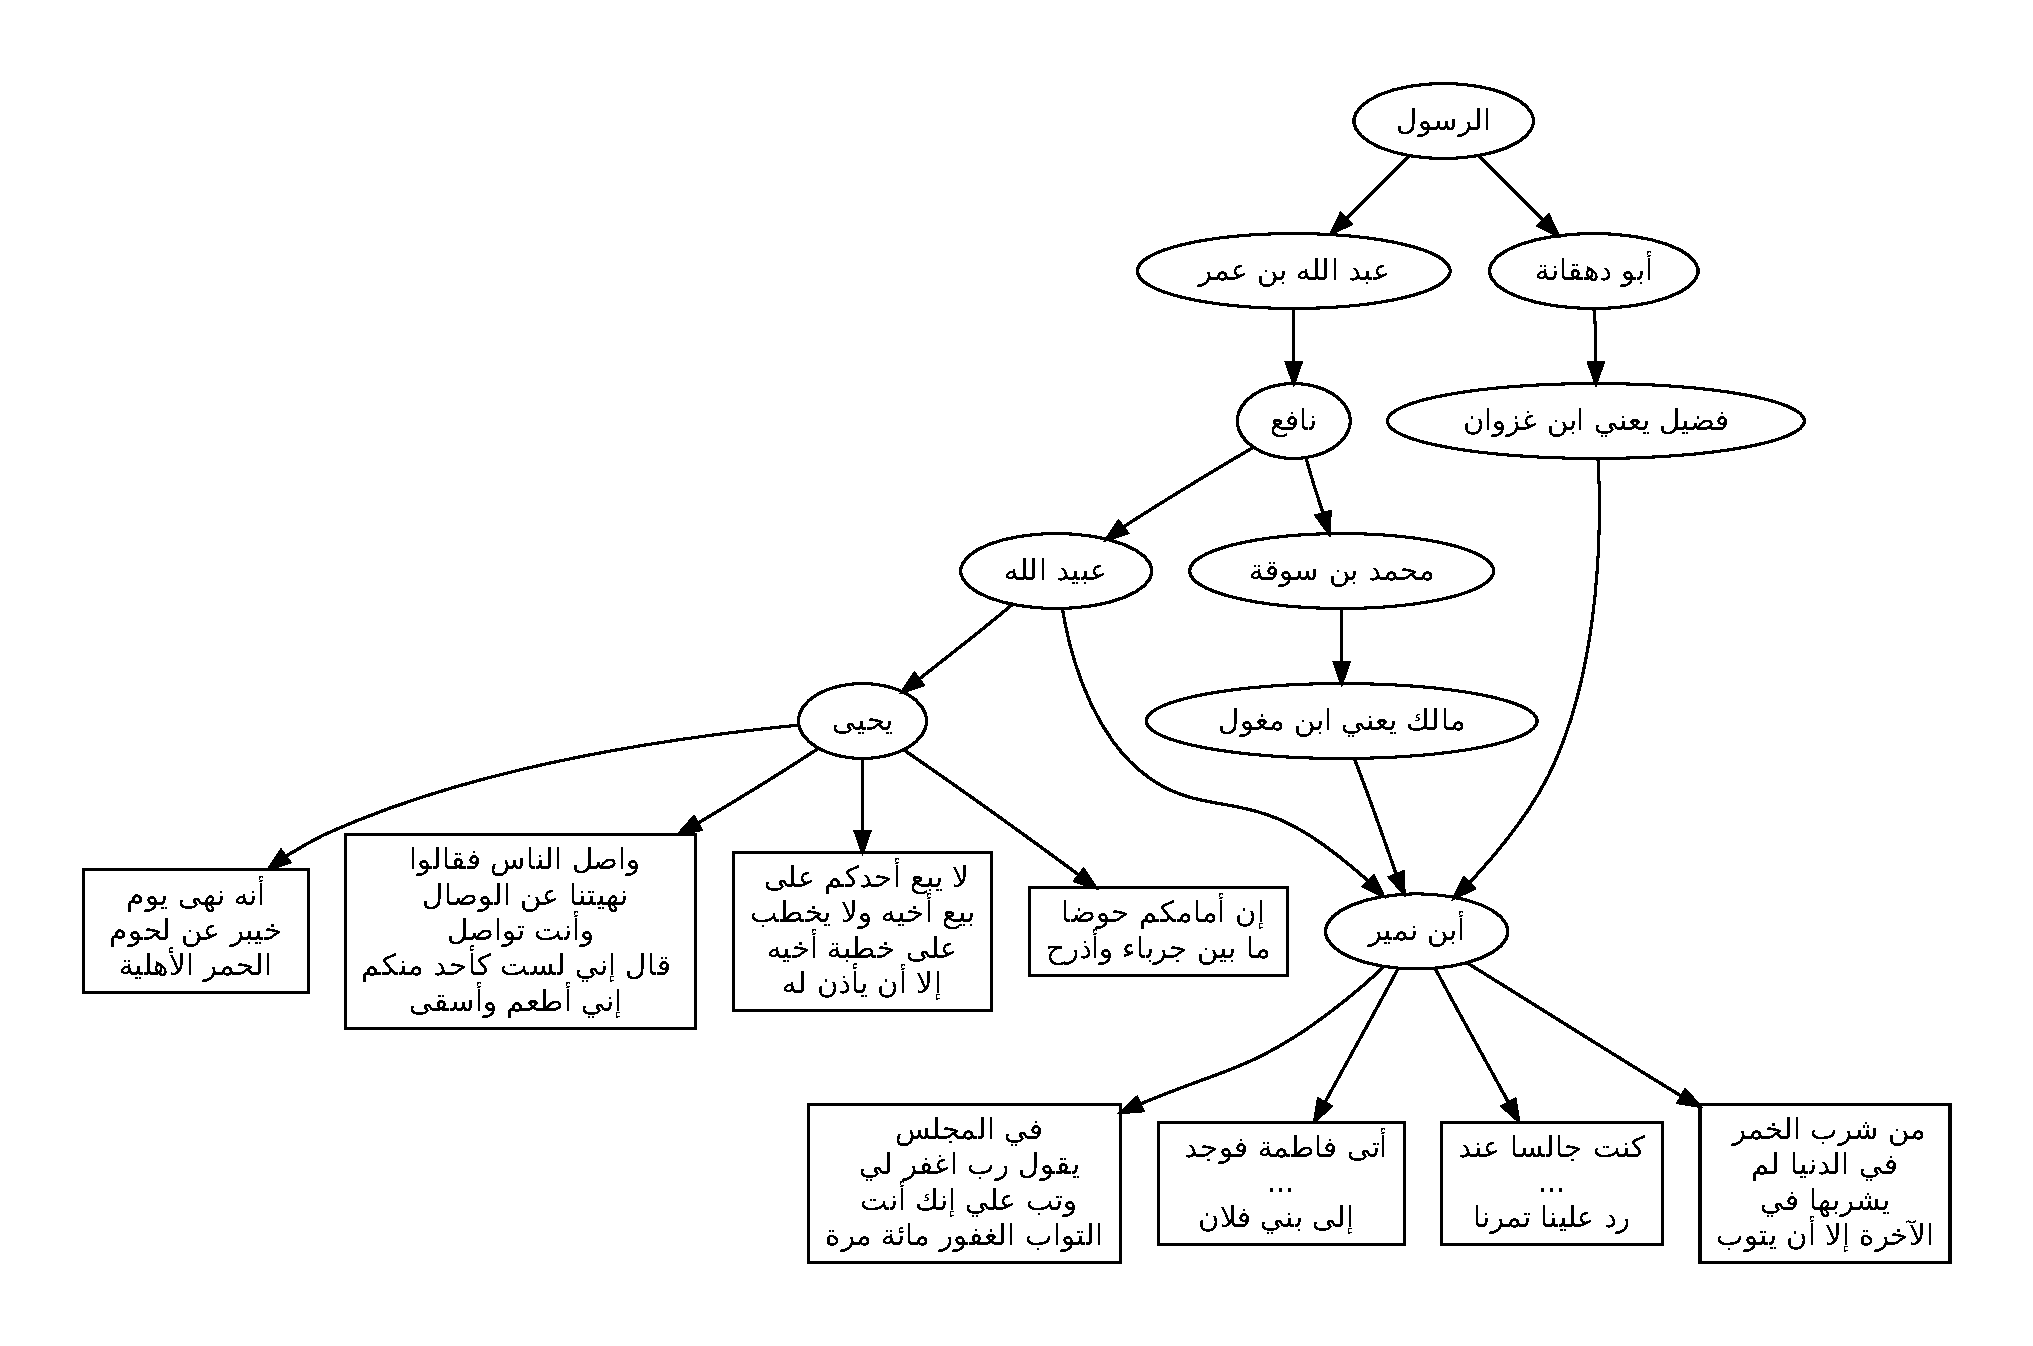
\includegraphics{figs/narrator_chain_output.pdf}
\label{f:narrators} } 
\caption{Directed acyclic graph representing a partial order 
    relation between narrators extracted using ATSarf}
}
\end{figure}

The directed acyclic graph (DAG) 
in Figure~\ref{f:narrators} shows a partial order relation (POR) between
narrators.
We automatically extracted the POR from hadith text 
documents.
The nodes in boxes are the \RL{matn} of the hadith, 
and the other nodes are the narrators.
Given a set of chains of narrators similar to 
Figure~\ref{f:exhadith} we formed the DAG using graph algorithms 
that merged equal names in the chains. 
This partial order graph is instrumental to automate
localizing narrators in biography documents and
segmenting biography documents.

Given that a biography will discuss a narrator and mention
his professors and students,
we can segment the biographies with a graph coloring algorithm 
that traverses the text and colors the POR whenever
a name is found. 
We modify the color when we move in the graph 
far away from the last name we colored.

Once the biographies are analyzed, one can annotate
the POR with qualifiers of the narrators that reflect
their authenticity. 
One can also annotate the POR with the locations and 
the time they lived in. 
Then One can compute a time and location overlap
check to discover inconsistent narrations.
We can also perform several interesting checks using 
this POR on its own such as checking for the effect of
one narrator on the hadith literature. 

These preliminary results serve as a good proof of concept to our 
hypothesis. They also confirm that our approach performs better than 
currently existing techniques from Sakhr~\cite{Sak09},
Basis~\cite{Bas09} and open source 
tools~\cite{Col09,Otakar:07,Tim04}.

We find evidence in our current results that features 
of the Arabic language such as the hierarchical structure of
names can be used to simplify the morphological analysis
needed to extract the partial order graph. 
Publications about these results are pending acceptance in 
related NLP conferences. 

The Co-Lead PI published extensively in this domain. 
A selected list of her recent publications follows. 
\begin{itemize}\itemsep0pt
\item Rehab Duwairi, Mohammad Al-Refai, Natheer Khasawneh, 
"Feature Reduction Techniques for Arabic Text Categorization". 
Journal of the American Society for Information Science and Technology 
(JASIST), Volume 60, Issue 11, pages: 2347-2352, 2009. 
\item Rehab M. Duwairi, "Arabic Text Categorization", 
International Arab Journal for Information Technology (IAJIT), 
Volume 4, Number 2, pages 125  132, 2007.
\item Rehab M. Duwairi, "Machine Learning for Arabic Text Categorization". 
Journal of the American Society for Information Science and Technology 
(JASIST), Vol. 57, Issue 8, pages 1005-1010, 2006.
\end{itemize}


%The Lead PI worked in the area of software arabization since 1996 
%as he worked on developing Arabization modules for Windows NT and 
%an 
%Arabic string manipulation library~\cite{Zar96}. 
%The Lead PI is also involved in working on an open source 
%project that aims at comprehensive automation of authenticity 
%checks against a corpus of literature heritage~\cite{Zaraket06}.
%The Lead PI is leading an effort at AUB to introduce 
%Computational Arabic in the curriculum of the ECE program. 
%He is also leading a team of students in an effort to place 
%the infrastructure needed for this project to start. 
%The lead PI worked and published about relational logic and 
%logic solvers applied to structured languages as follows.
%\begin{itemize}
%\item Sequential circuits for relational analysis. F. Zaraket, A. Aziz, and S. Khurshid. International Conference on Software Engineering, Minneapolis MN, 2007. 
%\item Sequential circuits for program analysis. F. Zaraket, A. Aziz, and S. Khurshid. Automated Software Engineering, Atlanta GA, 2007. 
%\end{itemize}

\section{Research design and methods}
\label{s:designmethods}

We see more and more Arabic documents such as texts,
books, publications, hospital and governmental records emerging 
every day.
Most of the newly generated documents are produced in digital 
textual form while also old paper documents are ported to digital 
form.
These documents include huge amounts of information that is 
qualitatively different than structured information such as that 
contained in database entries.
Text mining is the technology that automates the discovery of 
information in non structured text.

Text mining concerns the partitioning of text segments into classes,
the clustering of text segments,
the extraction of concepts and entities from text,
and the discovery and modeling of relations between text entities 
and classes.
Text mining techniques perform NLP to analyze text and perform 
IE to extract information into data structures.
Fundamental to IE are the named entity (NE) and the named entity 
relation (NER) extraction techniques which capture features from 
sentences and phrases.
A key challenge to NE and NER is that sentence structures and 
words are often ambiguous in natural languages.
%While research to address ambiguity in Latin languages is still 
%lagging behind~\cite{Red08},
%not much has been done to address NE and NER in the context of 
%the Arabic language.

The application of text mining techniques to Arabic text documents 
will result in great benefits to many research fields such as 
Arabic literature,
Islamic studies, Hadith authentication, and Arabic history and 
culture in general.
Arabic text mining will also benefit sectors where Arabic text 
documents are key such as the security sector,
the government personal records,
the taxation department,
the health sector,
as well as the trading floor of a stock exchange.
 
%The difficulty of applying text mining techniques to Arabic text 
%documents lays in the absence of automated tools that understand 
%the unique features of the Arabic language.
%We will make use of an example to illustrate the process.
Given an Arabic text document we want a tool that can segment 
and isolate all names, dates, time of the day occurrences,
tool names, and locations as entities.
Then we want another tool to identify relations amongst 
these entities such as identities and orders.
We want another tool to look at the verbs and actions in 
the sentences and try to build relations between the identified 
entities based on these verbs.
If we were successful to do that,
we now want to order all entities associated with dates based 
on a chronological order.

An order between two entities can depend on 
their simple order of appearance in the document, their 
numerical values in case they happened to be numbers, or
the distance between them in case they were cities. 
The relations can also be more sophisticated and 
based on templates provided by users or by 
models extracted from training data sets. 

To do the above, 
we need tools that automatically differentiate between 
names, verbs, adjectives and other structures.
This is not a simple task with the Arabic language.
For example, Arabic grammar allows name-based sentences 
or sentences with no verbs \noTrNoVocRL{^gml ismiyT} .
Another unique feature is the possibility to have names in Arabic 
that express action such as noun verbs 
\noTrNoVocRL{ism f`l, f-a`l $\ldots$}.

In addition to these structural differences,
there are features in the Arabic language that need special 
treatment such as derivatives and stems 
\noTrNoVocRL{alm^staq-at w al^g_dwr}.
Simple primitive tasks such as comparing two strings need 
special attention in Arabic since each Arabic letter has 
four different forms depending on its position in the word; 
isolated form, start, middle and end of a word.
Arabic diacritics should also be ignored most of the time 
when comparing two strings.
We also need to build dictionary tools that associate words 
and phrases based on their meanings and their context.
Often time,
and depending on the application and the user of the tool,
we need to allow the user to assign meanings and semantics 
for patterns in the text.

\subsection{Literature authentication case study}
\label{s:design:lit}

%\begin{figure}[tb]
\begin{figure}
\center{
\resizebox{.75\columnwidth}{!}
{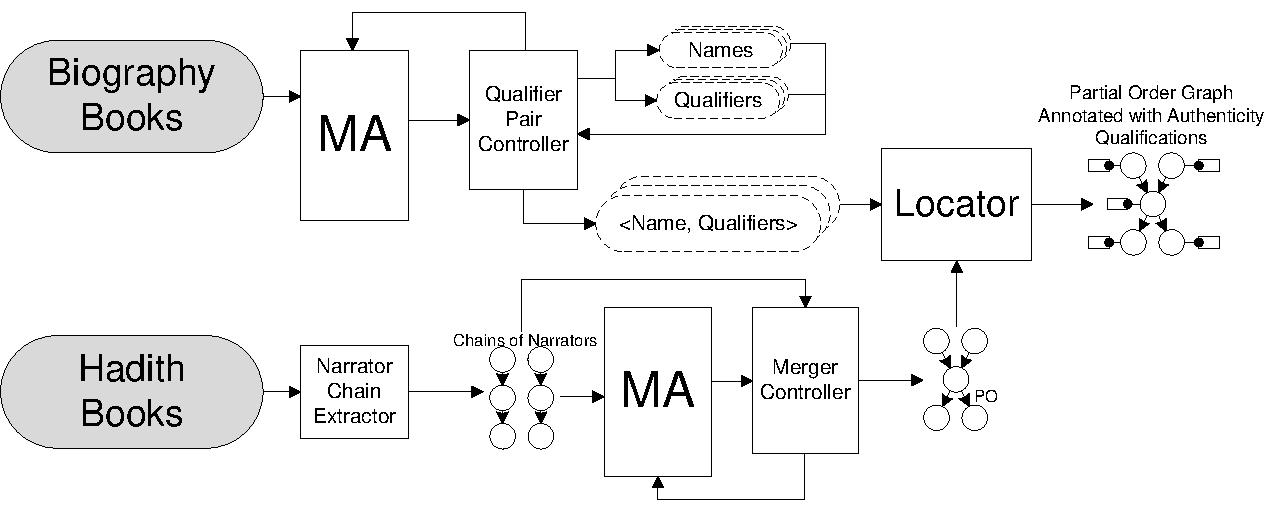
\includegraphics{figs/literature_case-study1.pdf}
\label{f:literature}
} 
\caption{CATARM diagram for the literature case study }
}
\end{figure}

The diagram in Figure~\ref{f:literature} describes our 
high level vision for what the literature case study
will look like in the CATARM framework. 
The boxes represent 
computational blocks provided by CATARM, 
ovals represent data blocks which are mainly the 
inputs and the outputs of the computational blocks. 
Dotted data blocks represent intermediate results,
and solid and shaded blocks represent the initial input 
and the final output respectively. 

The computational components can be direct CATARM components
or custom user components built from other CATARM components.
We feed the hadith books to a user Narrator Chain Extractor
component that we will discuss later in 
Section~\ref{s:design:chainext}. We  obtain a set of chains
of narrators that we feed to a morphological analyzer (MA) 
component controlled by a merger controller. 
The merger controller will look at the morphological analysis
of the narrator names and will decide to merge two narrators in 
one graph node in case they were morphologicaly equal. 
It will also give feedback to the MA component to stop the
analysis when a it reaches a satisfactory result.
We consider this graph as a partial order relation between 
narrators where a narrator precedes another narrator if 
he narrated from him. 

The biography books are fed to another MA unit controlled by 
a name and qualification pair controller that generates a 
map consisting of pairs of narrator names associated with 
qualifications. 
Then the graph of narrators and the narrator qualification map
are both processed through a locator component that computes
a graph coloring routine to color the graph of narrators. 
The color changes whener two consecutive narrators are far away
from each other in the text. 
The locator then looks at connected subgraphs of the same color,
and finds a median node in each of them to be the narrator 
associated with the qualifiers of the color. 
Then the locator also annotates the narrator with the 
corresponding qualifications. 
The result is an annotated partial order graph of narrators
with authentication qualification annotations. 

\subsection{Security case study}
\label{s:design:sec}

%\begin{figure}[tb]
\begin{figure}
\center{
\resizebox{.8\columnwidth}{!}
{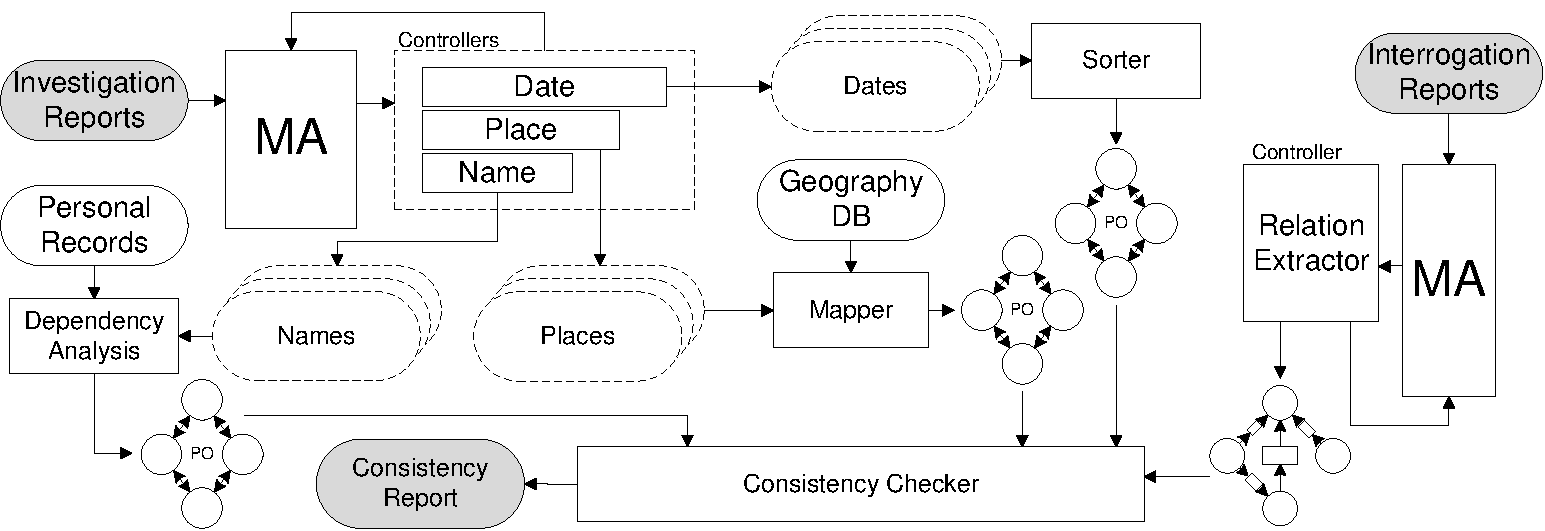
\includegraphics{figs/security_case-study.pdf}
\label{f:security}
}
\caption{CATARM diagram for the security case study}
}
\end{figure}


The diagram in Figure~\ref{f:security} describes our 
high level vision for what the solution of the 
security case study
will look like in the CATARM framework. 
The inputs are two separate sets of documents. 
The first set includes crime scene investigation reports, 
and the second set includes a 
interrogation reports with crime suspects as well as 
a database of previous interrogation reports. 
The CATARM system also takes as input a database of geographical
locations and a database of personal records. 
The aim is to check for inconsistencies in the iterrogation
reports and to identify possible connections between the suspects
and the crime scene. 

An MA with date, place, and name extraction controller extracts
names, dates and places from the investigation reports. 
We pass the dates to a sorting component to produce $G_D$ 
a partial order graph between the dates. 
We look up the names in the personal records database and find out
$G_N$ a family dependency graph between the names. 
We pass the places to a mapper that builds another $G_G$,
a graph relating the places using a geographical database. 

We pass the interrogation reports to an MA with a relation 
extraction controller that builds $G_R$. 
The graph $G_R$ relates the interrogated suspects
to each other, to places, and to dates based on a simple
neighborhood threshold computed using a statistical feature. 

We feed $G_D, G_F, G_G,$ and $G_R$   
to a consistency checker.
The consistency checker considers the three dimensions 
$N$ names, $G$ locations, and $D$ dates and projects $G_R$
over each one of them.
For each dimension $k$, it computes a local measure 
$\alpha_k$ of how much $G_R|_k$ simulates $G_k$. 
It flags the components in the graph where the accumelated 
measure $\alpha= \Sigma_{k\in\{D,N,G\}} \alpha_k$ is
below a threshold $\theta$ as inconsistent. 

\subsection{CATRAM components}
\label{s:design:components}

To do the above we need CATARM to provide us with several 
computational components such as a morphological analyzer, 
statistical tools, graph algorithms, and other computational
components. 
In the following we discuss the components needed for 
CATARM and we propose a methodology to 
use and extend existing tools, and develop new tools to
build the components of CATARM.

\subsection{Case-based morphological analyzer}

Morphological analyzers for the Arabic language
such as Buckwalter~\cite{Buckwalter:02},
Beesly~\cite{Beesley:01}, SAMA~\cite{Kulick:10},
and ElixirFM~\cite{Otakar:07} take an Arabic word as input
and produce several valid morpholgical solution for the word. 
Each solution is a sequence of morphemes that form the word.
Each morpheme is associated with several tags such as 
morphological, part of speech, grammar, and semantic tags. 
These analyzers are essential in several text analysis tools such 
as spell checkers as well as NLP frameworks~\cite{Col09}.
Other morphological analyzers such as 
Amira~\cite{Diab:07,Benajiba:07},
MAGEAD~\cite{Habash:05}, and MADA+TOKAN~\cite{Habash:09} 
use machine learning and support vector machines (SVM) 
to enhance the accuracy at the expense of efficiency.

The current use of morphological analyzers suffers from 
several problems. 
Analyzers that enumerate all possible partitions of a word
and match them against concatenative rules are computationaly 
expensive. 
Analyzers that exhaustively enumerate all possible solutions 
for a word may hurt performance and may
not be necessary or appropriate in some case studies~\cite{Maamouri:10}. 
For example, the first solution may be the one needed and 
we may not need to list the rest of the solutions. 
A white space delimited token may have more than one word
as is the case with ``run-on words''.

We propose to make use of the current existing morphological
analyzers to build a flexible and more efficient
morphological analyzer. 
The analyzer will be an essential
component in the CATARM framework. 
It will be a case-based analyzer as it will make guided decisions
based on feedback from the NLP case study and it will prune
invalid solutions on the fly. 

Case-based analysis can guide the morphological analysis
to prune lots of the solutions and to bias the order of considered
decisions. 
For example, in the hadith literature case study pesented above, 
amongst other things, we are intersted in checking whether a 
word is a name.  
We can bias the order of considered decisions to consider the 
morphemes that can be names first. 
If one of them matches, we can ignore the rest of the solutions. 
In case a prefix is decided to be of a morphological category
that does not connect with a name, then we can just ignore
the analysis of the rest of the word. 
This is more efficient than generating all possible partitionings
of the word, checking for morphological correctness of each 
partition, and then inspecting the part of speech tags of each
correct solution. 
We desire to build a morphological analyzer that allows a 
case-based controller to intervene at every single decision
without much overhead. 

\subsection{CATARM Query language}
\label{s:design:query}

We propose the CATARM query language with a user friendly
visual representation similar to that in Figures~\ref{f:literature} and
~\ref{f:security}. 
The basic elements in the query language will be entities, relations
and tags similar to those reported by a morphological analyzer. 
The query language will also have connectives such as set operations, 
relational operations, 
scalar and Boolean arithmetic operations, 
statistical computations, graph algorithms, and text algorithms
form terms and predicates that specify the desired computation
by the user. 
We will specify the CATARM query language in a formal grammar.

\subsection{Arabic linguistic computational model }
\label{s:design:lcm}

Several techniques~\cite{AEL07,Ham07,Abd07,MEl03} 
preprocessed the Arabic text and then used known text 
mining techniques that tend to Latin text and queries
to solve classification, indexing, named entity 
extraction and other problems.
We think that these techniques do not make use 
of Arabic language specific features.

We think that we can discover such features by building
a linguistic computational model of the Arabic language
based on its formal grammar and formal morphology
as defined in several Arabic linguistic 
sources~\cite{Sha73,Abd00,Abd001}.
We will build our morphological analyzer on top 
of this linguistic model in addition to the current existing
concatenative-based analysis techniques. 

Let $L_q$ be the query language grammar, 
$L_A$ be the grammar that expresses the Arabic linguistic
computational model, and let $q$ be a user query.
We compute $\rho_q$, the grammar path that matches 
the query $q$ in $L_q$. 
We will explore methods that use $\rho_q$ to simplify 
$L_A$ before we start the morphological analysis. 
We think the possible simplifications that we can perform
here are Language specific as they will reflect the 
correspondence between the formal query language definition $L_q$, 
the usage patterns of $L_q$  by Arabic users, 
and $L_A$ the formal LCM for Arabic. 


\subsection{Methodology}

\begin{figure}
\center{
\resizebox{.4\columnwidth}{!}
{\input{figs/hadith.pdftex_t}
\label{f:statemachine}
}
\caption{State-machine used to detect the chain of narrators}
}
\end{figure}

{\bf Case-based morphological analyzer.}
We experimented with several morphological analyzers.
We think that using finite state machines for morphological analysis
can be implemented in a more efficient way compared to other 
approaches. 
For example the concatenative rules used in Buckwalter~\cite{Tim04}
can be encoded in three FSM with linear execution time using 
the trie~\cite{datries} data structure. 

The use of FSMs also suits our case-based approach. 
The controller can be a FSM machine on its own and its decision
will be another input into the internal morphological FSM structures. 
This also suits our choice of enriching the concatenative analysis
with a formal linguistic model that can also be encoded into FSMs. 
FSM can also be easily integrated with hidden Markov models (HMM)
extracted from the sets of documents the MA will consider. 

The state machine in Firgure~\ref{f:statemachine} controls 
the concatenation based state machines of the morphological
analyzer.
The transitions are excited
by inputs from the morphological analyzer. 
A NAME label represents a proper name, 
an NRC label represents a narrator connector such as
\RL{`an} "on behalf of", \RL{qaal} "said", 
or one of their derivations. 
The IBN label corresponds to the word \RL{ibn} 
``the son of'' and represents a name connector.

The symbol $\tau_{\mbox{NMC}}$ is a threshold
that corresponds to the number of tolerated name connectors 
that may occur between two names. 
The symbol LIST$_{\mbox{NMC}}$ corresponds to the list 
of name connectors collected since the controller
started looping in the state NMC\_S. 
The symbol $\lambda_{\mbox{NMC}}$ is a parameter 
that corresponds to a relaxed tolerance measure that
the controller resorts to in case the words separating
two names were longer than $\tau_{\mbox{NMC}}$ but 
contained a name connector word such as IBN or NISBA.

The controller has four states that correspond to 
an abstract position in text relative to the next sanad. 
State TEXT\_S is the initial state and denotes that
the controller is outside the context of a sanad.
The controller moves to the state NAME\_S whenever
NAME is reported.
State NRC\_S means that the controller thinks it is in the context
of a narrator name after an NRC is reported.
State NMC\_S
indicates that the controller expects a name to appear within 
a tolerance threshold expressed by 
$\tau_{\mbox{NMC}}$ and $\lambda_{\mbox{NMC}}$.

Similarly, the NRC\_S state tolerates $\tau_{\mbox{NRC}}$ words 
before it gives up on its expectations. 

We reach the NAME\_S state only when a
valid NAME is detected and we leave when no more NAME's 
are detected. 
The NRC\_S state can only be reached if an NRC is detected.
NMC\_S can only be reached from a NAME\_S state.

The controller reports a valid chain of narrators when a 
sequence of names
connected by narrator connectors appears. 
It marks the beginning of the hadith with the beginning of the 
current sequence,
and marks the end of the hadith with the beginning of the next 
sequence. 
It also marks the chain of narrators as the sequence itself. 
The definition of input labels such as NAME and IBN depends on 
the morphological analyzer. 
We readily implemented the above approach and confirmed its 
accuracy and efficiency compared to existing morphological
analyzers. 

We will investigate enhancing our current case-based morphological
analyzer.
We will investigate methods to extend the internal structures 
of our analyzer to be able to represent a formal linguistic
computational model of the Arabic language. 

{\bf Linguistic computational model of Arabic.}
We think that a linguistic computational model for the Arabic
language will perform better in applications where
relations between Arabic text documents are involved. 
Such a model helps capture features unique and specific 
to the Arabic language and make use of that in the analysis.

ElixirFM~\cite{Otakar:07} builds on the lexicon
of the Buckwalter analyzer and the annotations of the 
Prague Arabic dependency databank to build a formal 
computational model of the Arabic language.
The models is a set of formulas and rules. 
ElixirFM uses the computational model in a functional
morphology framework that uses Haskell and functional
programming. 
The analyzer works by generating morphological trees of 
decisions and then uses a disambiguation decision procedure 
to annotate the trees with contextual elements. 

We will explore extracting our model from formal text book
definitions of the Arabic language~\cite{Abd00,Abd001} and seek
help from Arabic linguists to relax these formal rules to
allow common mistakes. 
We will encode the model in a grammar that we can synthesize
into an FSM and incorporate that with our current FSM 
morphological analyzer. 


{\bf User query language. }
In Figure~\ref{f:statemachine} we showed an FSM 
that controls the morphological analysis and generates a
list of chains of narrators out of hadith text.
We think that it is overwhelming to ask a user who is not 
versed in FSM and in computational sciences in general 
to design such a controller. 

The diagram in Figure~\ref{f:chain} depicts our vision of 
an equivalent query.
This query generates the list of chains by first passing the 
hadith text into the morphological analyzer which 
extracts names and their position in text. 
We iterate over the extracted names and compute the distance.
Whenever the distance is less than a threshold $\theta_1$
we add the word to a temporary chain of names. 
Otherwise, we execute a sequential block to 
{\bf 1.} tabulate the chain into a temporary table containing 
the list of chains. 
{\bf 2.} Create a new chain whith the last element.
Finally, we filter those chains whose cardinality 
is less than some threshold  $\theta_2$.

This query can be saved to a library of computational components
and invoked directly in another query 
as we saw in Figure~\ref{f:literature}.

\begin{figure}
\center{
\resizebox{.8\columnwidth}{!}
{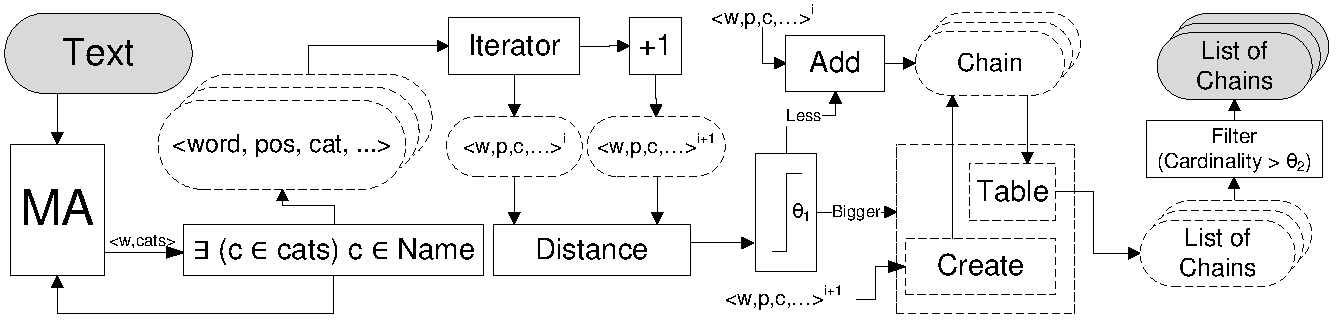
\includegraphics{figs/detailed_submachine.pdf}
\label{f:chain}
}
\caption{CATARM detailed diagram for the chain of narrators extractor}
}
\end{figure}

The CATARM query language will be expressed in a grammar 
where the atomic elements are user defined constants, or
entities and tags extracted by the morphological analyzer. 
The language will define terms, expressions, and predicates
using several connectives that express set operations, 
relational operations, Boolean operations, scalar operations, 
statistical tools, text algorithms, and graph algorithms. 
We need to provide a front end tool to support this query
language.

{\bf Simplify LCM based on the query.}
Given
L$L_q$ the query language, 
$L_A$ the Arabic linguistic
computational model, and  $q$ a user query
we compute $\rho_q$, the grammar path that matches 
the query $q$ in $L_q$. 
We plan to inspect methods to overapproximate 
the morphemes and the transitions in $L_A$ 
that can be satisfied by morphemes and transitions
in $\rho_q$. 
This can simplify the number of states we need to 
look at under $L_A$. 

This task is not trivial though, since $\rho_q$ may contain
states and transitions that are not always morphemes and 
transition between morphemes. 
We will consider a hierarchical methodology that follows 
the hierarchical structure of the Arabic language expressed
in $L_A$. For example,
we may consider sets of connected states in $\rho_q$ 
containing a single morpheme as a state in one hierarchy level 
in $L_A$.
We will perform this simplification before starting the 
morphological analysis since we already have to analyze
the query $q$ and compute $\rho_q$ before we start
the analysis. 

{\bf Simplify LCM and MA based on set of documents.}
We will analyze the set of input documents given to a
morphological analyzer component and use the analysis
to further improve the morphological analysis. 
We will extract statistical features from these documents 
to help order the solutions considered by the analyzer
to consider the most probable first. 

We will consider the use of HMM models 
built on the fly while processing the documents.
We will also consider the use of
latent semantic indexing~\cite{LSI89} techniques. 
We are considering these two techniques as they are 
both language independent and can both be computed and
adapted on the fly.

{\bf Entity and relational extractor.}
We will build a set of entity and relational extractors. 
The entities can be proper names, dates, locations,
and qualification adjectives. 
We will explore the use of pairing techniques to establish 
relations between the extracted entities.
The relations will form graphs as in the case studies presented
so far. The nodes represent the entities and the previously 
extracted relations and the edges represent the newly discovered 
relations.

The entity and relational extraction components 
may take as input a template for an expected relation and 
may return a graph that describes whether and where 
this relation exists between the subject documents.

We will need to augment the tags in the lexicons of the 
morphological analyzer to allow for better entity and relational
extractors. 
We plan to make use of existing annotated tree banks and of
modern Arabic dictionaries to do that. 

{\bf Statistical components.}
We will make use and build statistical components that can be used
in CATARM. 
We will need statistical components to rank solutions, compute 
probable decisions, estimating good thresholds. 

{\bf Graph algorithms.}
The relations extracted from the text documents will often 
be expressed in terms of graphs.
We will need textbook graph algorithms such as traversals, 
topological sorts, spanning trees, strongly connected 
components, minimum flow  and other algorithms.
For example, in the literature case study, the discovery
of articulation vertices may point to important narrators 
who may have an insignificant number of narrations 
but still connect narrator communities.

{\bf Query solver.}
This is a logical solver that will solve query expressions to \
resolve matching text and relations.
We will need to use existing off the shelf constraint solvers 
and set theory satisfiability solvers to address our queries. 
The solver should return and rank approximate matches.
That is if a three entities out of four required in a relation are
found, the solution is still worth reporting. 

The solver will call the morphological analyzer to compute 
morphological matches to the atomic elements of the query. 
Then each operation in the query such as a set intersection
operation will correspond to a computational component. 
The solver will call these components and integrate their
results. 

The solver may make use of existing propositional~\cite{MiniSAT} or
higher order logic~\cite{Z3} solvers if needed. 
These solvers can solve satisfiability questions.
We will explore the feasibility and utility 
of extracting a necessary set of 
constraints from the query and answering that with an off-the-shelf
logic solver. 

{\bf Case studies.}
We will work on developing the necessary components to complete 
the solution for the hadith literature and the security case 
studies.
We will also work on the health and network traffic case studies.
While working on the case studies, we will add the components
we build to our library of components. 
This will enrich CATARM with a useful set of computational 
components. 

{\bf Development methodology.}
We will integrate all the mentioned techniques in a scalable 
framework for Arabic text analysis.
The framework as a whole will allow for exhausting Arabic text 
analysis and allow for extensions of the framework.
A user should be able to iteratively and repetitively apply the 
abode techniques on his input text.

We will follow an eXtreme Programming 
methodology in the process of building CATARM.
We will use open source tools, libraries, and frameworks to 
build our libraries.
We will build on existing open source programming and text 
mining tools as well as open source Arabic text analysis tools 
based on NLP such as MADA+TOKAN~\cite{Rot08}, 
NEMLAR~\cite{RAl09}, and IJAES~\cite{Int09}.

We will use a dokuwiki based website~\cite{Dok09} 
to document the progress online and will use 
subversion~\cite{Sub09} as a source control tool.


 
{\bf Visualization.} 
We will build a visualization tool that allows fast 
and guided inspection and correction mechanism. 
The CATARM visualization aid will be a tag and relation color
sensitive browser.
The interface will allow a fast and guided inspection and 
correction mechanism.

\subsection{Research team}

\subsection{Work plan}

\subsection{Budget}


\section{Anticipated results and evaluation criteria}
\label{s:results}

We anticipate that the research will lead to the production of 
CATARM, an Arabic text analysis framework that allows relational 
queries between Arabic text documents.
The components of the framework are listed and discussed
in details in Section~\ref{s:design}. 

The following is a list of the anticipated components They are and are repeated for convenience as follows.
\begin{enumerate}
\item Case-based morphological analyzer 
\item Linguistic computational model for Arabic
\item User query language
\item Optimization methodologies
\begin{enumerate}
\item Use of language specific features 
\item Use of data in question specific features
\end{enumerate}
\item Entity and relational extractors
\item Statistical tools
\item Graph and text algorithms
\item Query solver
\item Case studies 
\begin{enumerate}
\item Hadith literature
\item Security
\item Health
\item Network content
\end{enumerate}
\end{enumerate}

\subsection{Evaluation Criteria}

The Lead PI will conduct biweekly meetings to track progress on the project.
 The team will maintain a dokuwiki based website to continuously post updates on the progress of the project.
 In Section "Research Design and Methods" we presented a schedule for delivering the different products of the project.
 The schedule can be used as a timeline for measuring the progress of the project.

The lexical and syntax analysis libraries will be compared with current open source libraries against commonly used corpora of data such as a collection of books or a collection of news reports.
 The dictionary module will be an augmentation over existing digitized dictionaries such as the Buckwalter~\cite{Tim04} morphological analyzer.
 In the entity and relational extraction tools we will use techniques native to the Arabic language and we will compare against English entity and relational extraction tools of similar or translated texts.
 We will also compare techniques that pre-process Arabic and then pass it to English IE and RE techniques.
 The logic solver will build over the IE and RE tools and will use off-the shelf quantifier and propositional solvers such as MiniSat~\cite{Een03}.
 The tagger is a GUI interface that allows fast manual inspection and refinement of the automated results.
 Each tool in the framework can start on its own with a prototypical implementation of the other needed tools.
 
Each tool in the framework stands alone and can operate on a well defined input and generate the desired output.
 The input of one tool, such as the entity extraction, can be automatically generated by another tool, such as the dictionary and the syntax analyzer.
  However, the input can also be manually generated if desired using the straightforward GUI tagger facility.
 Thus the tagger facility stands as a desired utility on its own and at the same time represents a contingency plan in case any module in the framework failed to deliver.
 
The team will publish the results of the research in the form of refereed conference and journal papers as well as tool papers addressing each of the tools.
 The team will also hold workshops to educate possible users on the tools once the tools are available.



\section{Strategy for project continuation}
\label{s:continue}


Once completed the Arabic text analysis framework will be an open source contribution and developers from the Arabic world in the open source community are expected to join efforts to keep it going.
 Furthermore, once completed the Arabic text analysis framework can sustain itself by charging on support or expert use.
 The framework or service on the framework can easily be commercialized to tend to the security, health, insurance, news, media, or literature business sectors.
 
The area of Arabic text analysis will be a research area for a long time as NLP is one of the most complex computational problems.
 The Arabic text analysis framework will be used by NLP researchers in the Arabic language field and those are expected to maintain and advance the framework.




\section{Plans for disseminating research results}
\label{s:dissem}

The team will publish the results of the research in the form 
of refereed conference and journal papers as well as tool papers 
addressing each of the tools. 
The team will also hold workshops to educate possible users on the 
tools once the tools are available.
The Arabic text analysis framework will be partially based on 
existing work in the open source domain and will thus be available 
as an open source tool. 
Interested researchers and users will be able to download the tools 
for free and use them for non-profit non-commercial purposes.  

\pagebreak
%\bibliography{adnan_refs}
%\bibliographystyle{ieeetr}
\bibliographystyle{abbrvnat}
%\bibliographystyle{ieeetr}
{\small
\bibliography{fzAr}  
}


\end{document}
